\label{ch:results}

\section{Overview}
\label{sec:results-overview}

This chapter reports full-scale evaluation results for all three Module~A generators specified in Chapter~\ref{ch:methodology} (Section~\ref{sec:module-a-crossmodel}): PRIMERA, LLM zero-shot, and LLM~+~retrieval. Each generator is evaluated on the identical 100 citation-dense Multi-LexSum test-split cases (Section~\ref{sec:eval-case-selection}), through the identical Module~B/C/correction pipeline, under the identical four conditions (Section~\ref{sec:conditions}). All three runs are complete at $n=100$; none of the numbers in this chapter are pilot or partial-run figures.

Results are organized by research question: RQ1 (Section~\ref{sec:results-rq1}), RQ2 (Section~\ref{sec:results-rq2}), RQ3 (Section~\ref{sec:results-rq3}), followed by a cross-generator comparison (Section~\ref{sec:results-crossgen}) and a qualitative error analysis (Section~\ref{sec:results-qualitative}).

\section{RQ1: Baseline Hallucination Profile}
\label{sec:results-rq1}

RQ1 asks what types and frequencies of case-citation hallucinations baseline summarizers produce under the CourtListener taxonomy (Table~\ref{tab:label-taxonomy}). Table~\ref{tab:rq1-labels} reports the label distribution eyecite and Module~C assign to each generator's uncorrected draft citations.

\begin{table}[!t]
\centering
\caption{RQ1: draft-citation label distribution by generator ($n=100$ cases each).}
\label{tab:rq1-labels}
\begin{tabular}{@{}lrrrrrr@{}}
\toprule
\textbf{Generator} & \textbf{Total} & \textbf{Verified} & \textbf{Mismatch} & \textbf{Ambiguous} & \textbf{NotFound} & \textbf{Baseline HR} \\
\midrule
PRIMERA          & 29  & 5 (17.2\%)   & 9 (31.0\%)   & 3 (10.3\%)   & 12 (41.4\%) & 82.8\% \\
LLM zero-shot     & 365 & 155 (42.5\%) & 58 (15.9\%)  & 94 (25.8\%)  & 58 (15.9\%) & 57.5\% \\
LLM + retrieval   & 689 & 203 (29.5\%) & 212 (30.8\%) & 215 (31.2\%) & 59 (8.6\%)  & 70.5\% \\
\bottomrule
\end{tabular}
\end{table}

No draft citation was ever labelled Malformed by any generator: eyecite's full-span extraction (Section~\ref{sec:module-b}) consistently produces parseable citation strings even when the underlying case does not exist.

Two findings are not visible from the headline HR percentage alone:

\paragraph{Citation-attempt density scales with generator, not with the task.} PRIMERA attempts 0.29 citations per case; LLM zero-shot attempts 3.65; LLM~+~retrieval attempts 6.89, roughly an order of magnitude more than PRIMERA in both LLM-based conditions. This is the citation-coverage question raised in Section~\ref{sec:module-a-crossmodel}: PRIMERA's 29 total citations against 631 in the matching gold summaries could have reflected either a property of legal case summarization or an artefact of one checkpoint's short-output ceiling. Both LLM-based generators resolve this in favour of the latter: nothing about the task itself suppresses citation attempts to PRIMERA's degree.

\paragraph{The label profile, not just the count, changes with generator.} PRIMERA's few attempted citations skew NotFound (41.4\%), consistent with a short, compressed draft naming cases only in passing, with a high chance the citation is simply invented rather than a near-miss on a real one. LLM zero-shot's citations skew Verified (42.5\%): the model attempts many citations and roughly two in five resolve cleanly. LLM~+~retrieval's citations are the most evenly spread across Verified/Mismatch/Ambiguous (29--31\% each) and have the \emph{lowest} NotFound rate of the three (8.6\%): ranking source material by citation density before truncation does not only increase how many citations the model attempts, it increases the fraction of those attempts that resolve to \emph{some} real case, even when the specific match is wrong (Mismatch) or contested (Ambiguous). Retrieval measurably improves what fraction of attempts land near a real citation, rather than simply adding more noise.

\section{RQ2: Effect of Symbolic Verification and Correction}
\label{sec:results-rq2}

RQ2 asks whether symbolic verification plus bounded correction measurably reduces paired citation hallucination rate relative to the neural-only baseline. Table~\ref{tab:rq2-results} reports paired HR before and after the symbolic condition, the relative reduction, and McNemar significance for each generator.

\begin{table}[!t]
\centering
\caption{RQ2: paired HR before/after symbolic correction, by generator ($n=100$).}
\label{tab:rq2-results}
\begin{tabular}{@{}lrrrrr@{}}
\toprule
\textbf{Generator} & \textbf{Baseline HR} & \textbf{HR after correction} & \textbf{Relative reduction} & \textbf{Fix rate} & \textbf{McNemar $p$} \\
\midrule
PRIMERA         & 82.8\% & 27.6\% & 71.8\% & 31.0\% & $3.05\times10^{-5}$ \\
LLM zero-shot    & 57.5\% & 22.2\% & 56.1\% & 61.9\% & $2.94\times10^{-39}$ \\
LLM + retrieval  & 70.5\% & 24.2\% & 65.9\% & 64.9\% & $1.87\times10^{-96}$ \\
\bottomrule
\end{tabular}
\end{table}

\begin{figure}[!t]
\centering
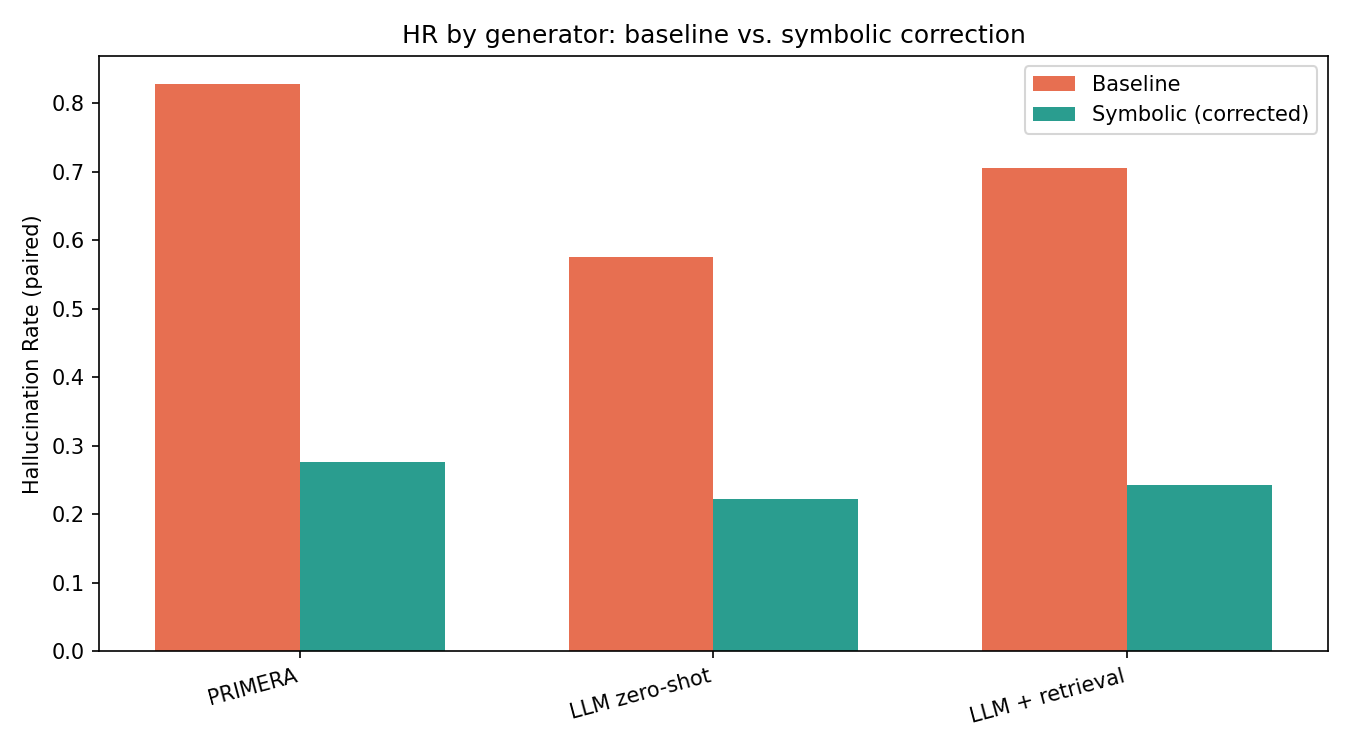
\includegraphics[width=0.85\linewidth]{hr_by_generator.png}
\caption{Paired HR by condition, all three generators, same 100 cases. Baseline (crimson) vs.\ symbolic correction (teal).}
\label{fig:hr-by-generator}
\end{figure}

All three reductions are significant well beyond conventional thresholds. More importantly, McNemar's discordant-pair counts (Table~\ref{tab:rq2-discordant}) show the same qualitative pattern in every generator: many citations flip from hallucinated to resolved, and \emph{zero} flip the other way.

\begin{table}[!t]
\centering
\caption{McNemar discordant pairs by generator: citations that flipped outcome under correction.}
\label{tab:rq2-discordant}
\begin{tabular}{@{}lrrr@{}}
\toprule
\textbf{Generator} & \textbf{Paired citations} & \textbf{Bad $\rightarrow$ fixed} & \textbf{Fixed $\rightarrow$ bad} \\
\midrule
PRIMERA         & 29  & 16  & 0 \\
LLM zero-shot    & 365 & 129 & 0 \\
LLM + retrieval  & 689 & 319 & 0 \\
\bottomrule
\end{tabular}
\end{table}

Across all three generators and 1{,}083 paired citations, correction never converts a citation that was already acceptable into a hallucination. This is a direct consequence of the safety-first correction policy (Section~\ref{sec:correction}): repair only fires when Module~C resolves a citation without a hard party contradiction, Ambiguous spans are left flagged or re-anchored rather than guessed, and the policy never substitutes a contradicting case name. The zero-regression result is the empirical payoff of that conservatism, not a coincidence of one favourable run, but a pattern that reproduces identically across three architecturally different generators with very different starting HRs (82.8\% down to 57.5\%) and citation volumes (29 up to 689).

Fix rate, the share of draft citations repaired in place rather than redacted, also tracks generator, not just outcome HR: PRIMERA repairs 31.0\% of its citations and redacts the rest (its removal rate is 41.4\%, the highest of the three), while both LLM-based generators repair roughly two-thirds of theirs (61.9\%, 64.9\%) and redact under 16\%. With only 29 total citations, a larger share of PRIMERA's failures are citations Module~C cannot resolve to any case at all (NotFound, Table~\ref{tab:rq1-labels}) rather than near-misses on a real one: NotFound citations are always redacted, never repaired, by policy (Table~\ref{tab:label-taxonomy}).

\section{RQ3: Quality Preservation Under Correction}
\label{sec:results-rq3}

RQ3 asks whether the full generate--verify--correct pipeline can preserve summary quality while reducing paired HR by at least 30\% relative to baseline. Both criteria are evaluated independently; Table~\ref{tab:rq3-results} reports the primary quality metric, ROUGE-L\textsubscript{sum} (Section~\ref{sec:method-metrics}), before and after symbolic correction, alongside BERTScore F1.

\begin{table}[!t]
\centering
\caption{RQ3: quality metrics before/after symbolic correction, by generator ($n=100$). Both are scored against the expert gold summary, not against each other (Section~\ref{sec:method-metrics}).}
\label{tab:rq3-results}
\begin{tabular}{@{}lrrrrr@{}}
\toprule
\textbf{Generator} & \textbf{ROUGE-L\textsubscript{sum} before} & \textbf{after} & \textbf{$\Delta$ (pp)} & \textbf{BERTScore F1 before} & \textbf{after} \\
\midrule
PRIMERA         & 0.4074 & 0.4069 & $-0.05$ & 0.8511 & 0.8508 \\
LLM zero-shot    & 0.4251 & 0.4252 & $+0.00$ & 0.8331 & 0.8329 \\
LLM + retrieval  & 0.4303 & 0.4295 & $-0.07$ & 0.8347 & 0.8345 \\
\bottomrule
\end{tabular}
\end{table}

Every delta is far inside the $\pm 2$ percentage-point tolerance, by roughly two orders of magnitude. Bootstrap 95\% confidence intervals on the paired delta (1{,}000 resamples) confirm this is not an artefact of averaging: PRIMERA $[-0.090\%, -0.020\%]$, LLM zero-shot $[-0.070\%, +0.093\%]$, LLM~+~retrieval $[-0.131\%, -0.012\%]$; every interval sits within a fraction of a percentage point of zero, and none crosses the tolerance boundary in either direction. BERTScore F1 moves by at most 0.0003 in any condition.

\begin{table}[!t]
\centering
\caption{RQ3 pass/fail summary, both criteria, all three generators.}
\label{tab:rq3-pass}
\begin{tabular}{@{}lrrcc@{}}
\toprule
\textbf{Generator} & \textbf{HR reduction} & \textbf{ROUGE-L\textsubscript{sum} $\Delta$} & \textbf{HR target ($\geq 30\%$)} & \textbf{Quality target ($\leq \pm 2$pp)} \\
\midrule
PRIMERA         & 71.8\% & $-0.05$pp & PASS & PASS \\
LLM zero-shot    & 56.1\% & $+0.00$pp & PASS & PASS \\
LLM + retrieval  & 65.9\% & $-0.07$pp & PASS & PASS \\
\bottomrule
\end{tabular}
\end{table}

RQ3 is answered affirmatively for all three generators, not only for the strongest case. This matters for the claim's generality: the smallest HR reduction observed (LLM zero-shot, 56.1\%) is still $1.87\times$ the 30\% target, and the largest quality cost observed (LLM~+~retrieval, $-0.07$pp) is $1/28$\textsuperscript{th} of the $\pm2$pp tolerance. The two stay close to orthogonal in this pipeline, rather than trading off at a rate that happens to clear the bar, because symbolic correction edits only the character spans eyecite identified as citations (Section~\ref{sec:module-b}), typically a few dozen characters inside a summary of several hundred words, and leaves the surrounding prose untouched.

\subsection{Why plain ROUGE-L is not the reported gate}
\label{sec:results-rougeL-note}

An earlier pass through this evaluation reported plain ROUGE-L (single LCS over the entire flattened summary) rather than ROUGE-L\textsubscript{sum} (sentence-split, union-LCS), because \texttt{rouge\_score}'s \texttt{rougeLsum} implementation silently collapses to plain ROUGE-L when the input text contains no newlines, which draft and gold summaries here do not, by default. Plain ROUGE-L is not the variant Multi-LexSum's own reported PRIMERA baseline uses (Table~\ref{tab:relatedwork}: ROUGE-L $30.89$), and is not standard practice for multi-sentence summarization evaluation, where a single global LCS heavily penalizes any sentence-order variation that does not affect faithfulness. Table~\ref{tab:rougeL-variant-diff} shows both variants side by side on this evaluation's own PRIMERA baseline drafts: plain ROUGE-L sits roughly $17$ points below Multi-LexSum's published figure, while ROUGE-L\textsubscript{sum}, computed identically except for sentence splitting before scoring, sits above it.

\begin{table}[!t]
\centering
\caption{Plain ROUGE-L vs.\ ROUGE-L\textsubscript{sum} on the same PRIMERA baseline drafts ($n=100$), against the published Multi-LexSum PRIMERA baseline.}
\label{tab:rougeL-variant-diff}
\begin{tabular}{@{}lrr@{}}
\toprule
& \textbf{This evaluation} & \textbf{Multi-LexSum PRIMERA baseline} \\
\midrule
Plain ROUGE-L      & 0.1995 & 0.3089 \\
ROUGE-L\textsubscript{sum} & 0.4074 & --- \\
\bottomrule
\end{tabular}
\end{table}

Both variants are computed by the same evaluation harness and reported in every table in this chapter (Section~\ref{sec:method-metrics}); this section documents the correction so the two numbers are not mistaken for a regression. Critically, the RQ3 conclusion is unaffected by which variant is used as the gate: the before/after delta is near-zero under both (Table~\ref{tab:rq3-results} vs.\ the plain-ROUGE-L deltas of $-0.0005$pp, $+0.03$pp, $+0.01$pp for PRIMERA, LLM zero-shot, and LLM~+~retrieval respectively), because the correction policy's edits are too localized to move either LCS-based metric meaningfully. What the variant choice affects is only the \emph{absolute} number's comparability to the literature, not the paired-comparison conclusion this thesis draws from it.

\section{Cross-Generator Comparison}
\label{sec:results-crossgen}

Sections~\ref{sec:results-rq1}--\ref{sec:results-rq3} answer RQ1--RQ3 once per generator; this section asks what changes, and what does not, across generators.

\begin{figure}[!t]
\centering
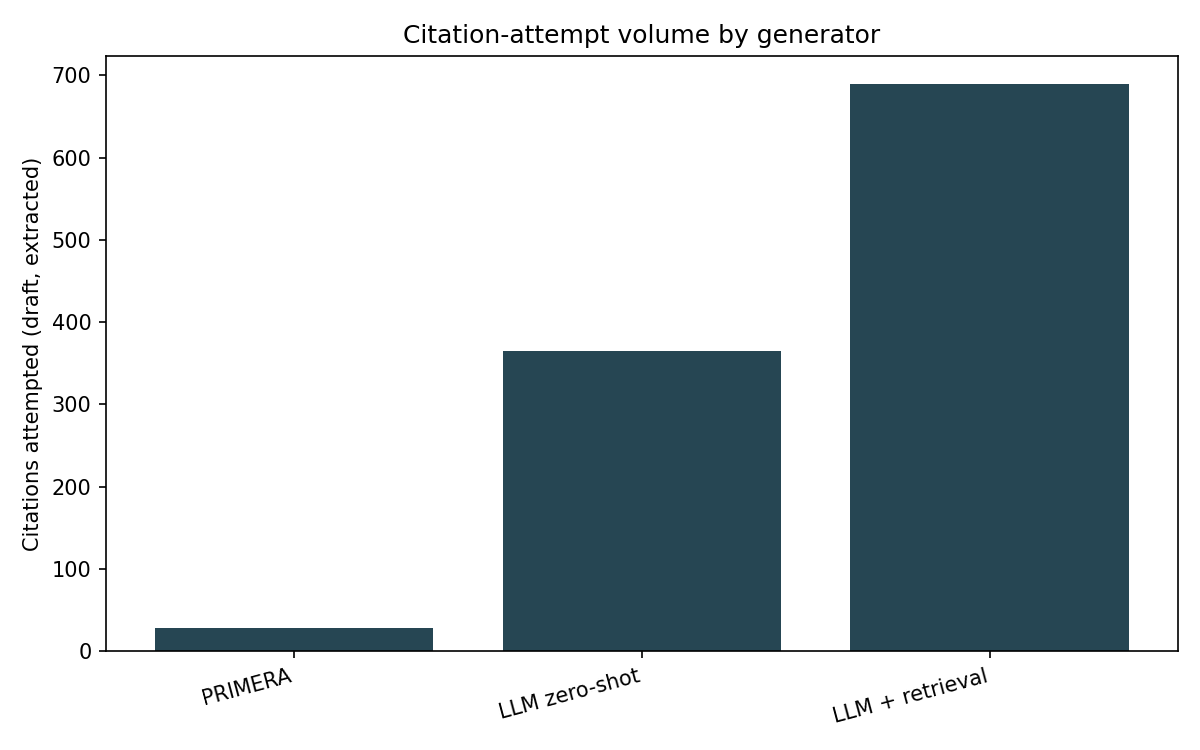
\includegraphics[width=0.85\linewidth]{citations_attempted_by_generator.png}
\caption{Citations attempted per draft (summed across 100 cases) vs.\ the gold-summary reference count (631), by generator.}
\label{fig:citations-attempted}
\end{figure}

\paragraph{The correction pipeline generalizes across generator architecture.} Final paired HR lands in a narrow band (27.6\%, 22.2\%, 24.2\%) despite baseline HRs that differ by 25 percentage points (82.8\% down to 57.5\%) and citation volumes that differ by $24\times$ (29 up to 689). Module~C and the correction policy were designed and tuned against PRIMERA's low-volume, NotFound-heavy citation profile; nothing in the policy is generator-specific, and the LLM-based conditions, high-volume, Verified/Mismatch/Ambiguous-heavy, were not available during that design process, since they were added specifically to test whether PRIMERA's profile was representative (Section~\ref{sec:module-a-crossmodel}). The pipeline was not implicitly overfit to the case it was built against.

\paragraph{Retrieval's effect is a net positive, with a visible trade-off.} Ranking source documents by citation density before truncation (the LLM~+~retrieval variant) raises baseline HR relative to naive truncation (70.5\% vs.\ 57.5\% for LLM zero-shot): more attempted citations surface more borderline cases, not only easy ones, consistent with Section~\ref{sec:results-rq1}'s finding that retrieval also shifts the label mix toward Mismatch/Ambiguous. But retrieval simultaneously nearly doubles citation-attempt density (6.89 vs.\ 3.65 per case) and, after correction, achieves both a larger absolute quantity of successfully-resolved citations (319 fixed, Table~\ref{tab:rq2-discordant}) and a final HR statistically indistinguishable from the non-retrieval LLM condition. Retrieval trades a higher pre-correction failure rate for substantially more real citation coverage, and the correction stage absorbs the difference.

\section{Qualitative Error Analysis}
\label{sec:results-qualitative}

Aggregate metrics do not show \emph{how} a generator fails. One failure mode recurs often enough across the LLM-based conditions to warrant a worked example and a corpus-wide count: a generator fabricating a run of near-identical citations to the same case, varying only the reporter volume, page, and year.

\paragraph{Worked example.} Case \texttt{CJ-AZ-0002} under the LLM zero-shot condition drafted 25 separate citation attempts to \emph{Wood v.\ Ryan}, an actual Ninth Circuit party pair, but with fabricated reporter details: F.3d volume numbers increasing by roughly 14 with each attempt (851, 876, 895, 917, \ldots, 1223), the page number fixed at 1098 throughout, and years drifting from 2017 to 2022 with no consistent pattern. Exactly one of these 25 attempts (volume 851, year 2017) resolved to a real, Verified case; Module~C labelled the rest Ambiguous or NotFound, and the correction policy redacted 22 of them and left 2 Ambiguous spans flagged rather than guessing among the fabricated volumes (Table~\ref{tab:label-taxonomy}). Draft paired HR for this single case was 0.839; after correction it fell to 0.065.

\paragraph{The same case across all three generators.} \texttt{CJ-AZ-0002} is the one case ID that appears in every generator's review export, so it is also the one case where PRIMERA, LLM zero-shot, and LLM~+~retrieval can be compared directly rather than across different source material. Figure~\ref{fig:sample-case-dashboard} shows the outcome. PRIMERA drafts only 2 citations for this case (both unverified at draft time; correction fixes 1 of 2). LLM zero-shot drafts 31, dominated by the Wood~v.\ Ryan run above, and correction resolves all but 2. LLM~+~retrieval drafts 6, of which 3 verify immediately and 3 remain Ambiguous with no safe anchor, so correction leaves the case unchanged (HR stays at 0.5). The same source docket produces a citation-attempt count that differs by more than $15\times$ across generators, and a correction outcome that ranges from complete resolution to no resolution at all, depending on which generator drafted the citations Module~C had to work with.

\begin{figure}[!t]
\centering
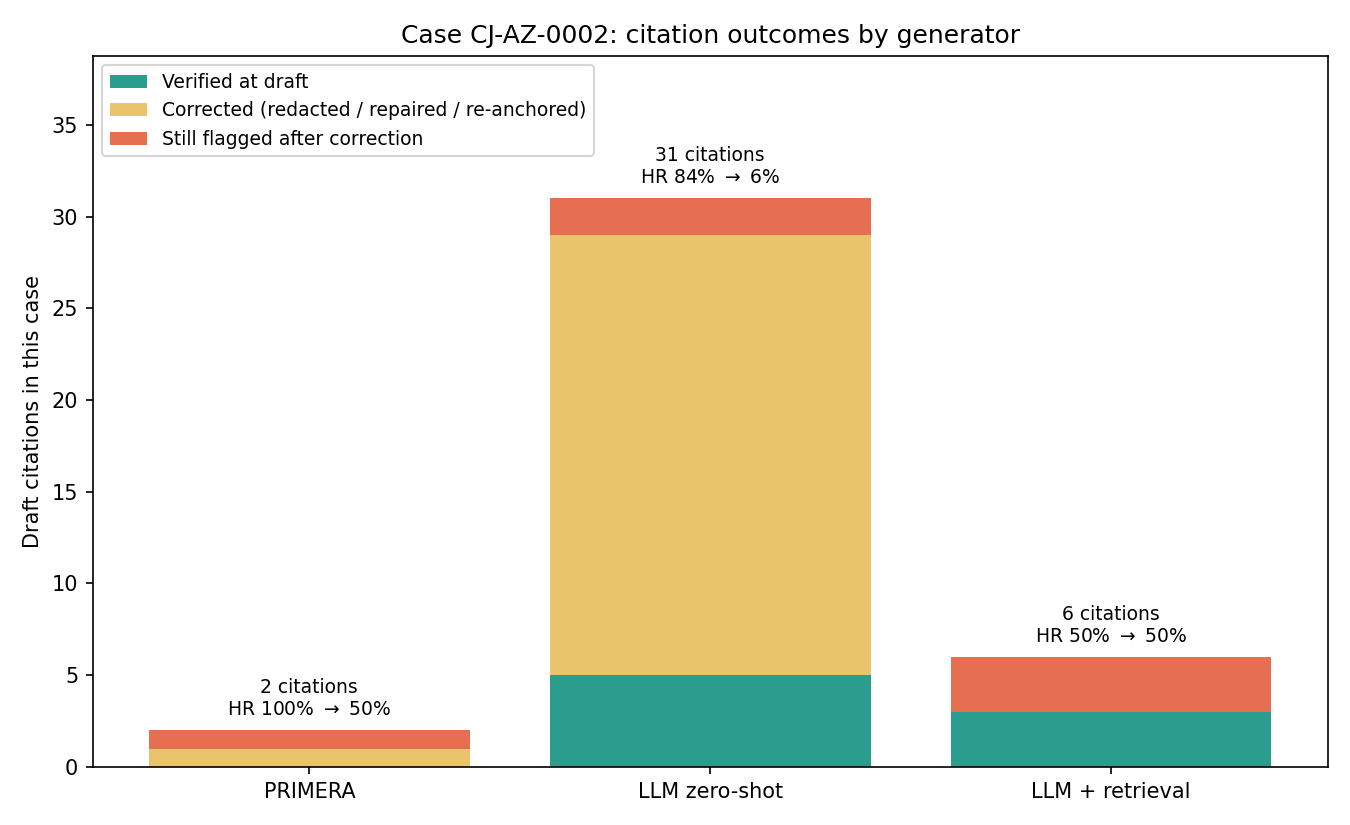
\includegraphics[width=0.85\linewidth]{sample_case_dashboard.png}
\caption{Case \texttt{CJ-AZ-0002}: draft citation outcomes by generator. Each bar is the total draft citations for this one case, split into citations already Verified at draft time, citations the correction policy resolved (redacted, repaired, or re-anchored), and citations still flagged after correction.}
\label{fig:sample-case-dashboard}
\end{figure}

\paragraph{Prevalence.} Treating five or more citations to the same case name within one draft as a degenerate run, Table~\ref{tab:degenerate-runs} quantifies how often this pattern occurs across all 100 cases, by generator.

\begin{table}[!t]
\centering
\caption{Degenerate same-case citation runs ($\geq 5$ citations to one case name in a single draft), by generator.}
\label{tab:degenerate-runs}
\begin{tabular}{@{}lrrr@{}}
\toprule
\textbf{Generator} & \textbf{Citations in degenerate runs} & \textbf{Share of total} & \textbf{Cases affected} \\
\midrule
PRIMERA         & 0  & 0.0\%  & 0 / 100 \\
LLM zero-shot    & 50 & 13.7\% & 4 / 100 \\
LLM + retrieval  & 5  & 0.7\%  & 1 / 100 \\
\bottomrule
\end{tabular}
\end{table}

PRIMERA's short, extractive-leaning drafts never exhibit this pattern, consistent with its low overall citation-attempt rate (Section~\ref{sec:results-rq1}). LLM zero-shot is the most affected: 13.7\% of its 365 citations sit inside degenerate runs, concentrated in 4 of 100 cases (the worst being the \emph{Wood v.\ Ryan} example above). LLM~+~retrieval, despite attempting nearly double the citations per case of LLM zero-shot, shows the pattern in under 1\% of its citations and only 1 case: source documents ranked by citation density appear to give the model enough real citation material that it does not need to extrapolate a fabricated sequence to satisfy an instruction to cite sources. This is a second, independent piece of evidence for retrieval's benefit beyond the aggregate HR numbers in Section~\ref{sec:results-crossgen}: the specific \emph{failure mode} of runaway fabrication is largely suppressed, not just the count of attempted citations that resolve successfully.

In every case in Table~\ref{tab:degenerate-runs}, the correction policy handled the degenerate run correctly by construction: each fabricated citation is verified independently, so a NotFound or Ambiguous label triggers redaction or flagging regardless of how many similar-looking fabrications preceded it in the same draft. No special-case handling for repetition was needed; this is a direct consequence of Module~C treating every extracted citation as an independent claim to check (Section~\ref{sec:module-c}), rather than summarizing or deduplicating across a draft before verification.

\section{Chapter Summary}
\label{sec:results-summary}

All three research questions are answered affirmatively for all three generators evaluated:

\begin{itemize}
  \item \textbf{RQ1:} Baseline citation hallucination is substantial in every generator (57.5--82.8\% paired HR) but its character differs sharply by generator: PRIMERA's few citations skew NotFound; LLM-based generators attempt an order of magnitude more, and retrieval further shifts the mix toward resolvable (if not always correct) matches.
  \item \textbf{RQ2:} Symbolic verification and bounded correction reduce paired HR by 56.1--71.8\% relative to baseline, with McNemar significance below $10^{-4}$ in every generator, and, across all 1{,}083 paired citations in this evaluation, \emph{zero} citations were ever made worse by correction.
  \item \textbf{RQ3:} Quality is preserved with wide margin in every generator: ROUGE-L\textsubscript{sum} moves by at most 0.07 percentage points against a $\pm2$pp tolerance, and BERTScore F1 by at most 0.0003.
\end{itemize}

The cross-generator comparison shows the correction pipeline generalizes rather than having been implicitly tuned to PRIMERA's citation profile, and the qualitative analysis identifies a specific fabrication failure mode, degenerate same-case citation runs, that citation-density retrieval substantially, though not completely, suppresses. The following chapters interpret these findings against the research gap and literature (Chapter~\ref{ch:lit-review}) and state the thesis's contributions, limitations, and open work.
